
\normalsize Le definizioni di acidi e basi sono variate negli anni.

Inizialmente abbiamo classificato come acido o base un dato composto in funzione dell'elettronegatività dell'atomo X nella seguente reazione

$$\ce{XOH(aq) + H_2O -> XO^-(aq) + H_3O^+(aq)}, \quad \text{X elettronegativo}$$

$$\ce{XOH(aq) + H_2O -> X^+(aq) + OH^-(aq)}, \quad \text{X elettropositivo}$$

Immaginiamo quindi di avere un generico composto formato da un atomo X con almeno un gruppo OH.

Alcuni composti liberano il loro idrogeno sotto forma di H$^+$, cioè in essi si rompe il legame ossigeno-idrogeno, altri invece liberano il gruppo O-H sotto forma di OH$^-$, cioè si rompe il legame X-OH. Quindi in funzione dell'elettronegatività dell'atomo X si può vedere quale sia il legame più facile da rompere in acqua:

\begin{itemize}
    \item Se il composto libera ioni H$^+$ diciamo che è \textbf{acido}.
    \item Se il composto libera ioni OH$^-$ diciamo che è una \textbf{base}.
\end{itemize}

\subsection{Definizione di Arrhenius (1887)}
La definizione finora adoperata è stata enunciata da Arrhenius, il quale etichettò come acido una qualunque specie chimica che in acqua libera ioni H$^+$ e come base una qualunque specie chimica che in acqua libera ioni OH$^-$.

\vspace{0.2cm}Esempi di acidi:

\vspace{0.2cm}\ce{HCl(aq) + H_2O -> H^+(aq) + Cl^-(aq)}

\vspace{0.2cm}\ce{H_2SO_4(aq) + H_2O -> H^+(aq) + H_2SO_4^-}

\vspace{0.2cm}\ce{H_2SO_4^- + H_2O -> H^+(aq) + SO_4^{2-}}

\vspace{0.2cm}Esempi di basi:

\vspace{0.2cm}\ce{NaOH(aq) -> Na^+(aq) + OH^-(aq)}

\vspace{0.2cm}\ce{Ba(OH)_2(aq) -> Ba(OH)^+(aq) + OH^-(aq)}

\vspace{0.2cm}\ce{Ba(OH)^+ -> Ba^{2+}(aq) + OH^-(aq)}

\vspace{0.2cm}Questa definizione però pone due limiti:

\begin{enumerate}
    \item Si considera solo l'acqua come solvente, per cui se questi composti fossero in solventi diversi non avremmo modo di etichettarli;
    \item Ci sono delle incongruenze. Ad esempio l'ammoniaca NH$_3$ che è una base non ha ioni OH$^-$ da liberare, pertanto secondo questa definizione non potrebbe essere una base.
\end{enumerate}
\subsection{Definizione di Brönsted-Lowry (1923)}
Si giunse quindi alla teoria acido-base di Brönsted-Lowry. Con essa si etichetta acido ogni specie chimica che è in grado di donare protoni.

\vspace{0.2cm}Esempi di acidi di Brönsted-Lowry:

\vspace{0.2cm}\ce{CH_3COOH(aq) + H_2O <--> CH_3COO^-(aq) + H_3O^+}

acido acetico \hspace{2.55cm} ione acetato 

\vspace{0.2cm}\ce{NH_4^+(aq) + H_2O <--> NH_3(aq) + H_3O^+(aq)}

ione ammonio \hspace{1.35cm} ammoniaca

\vspace{0.2cm}\ce{H_2PO_4^-(aq) + H_2O <--> H_2PO_4^{2-}(aq) + H_3O^+(aq)}

ione fosfato \hspace{2.25cm} ione fosfato

acido \hspace{3.4cm} bi-acido

\vspace{0.2cm}Lo ione H$^+$ è scritto come H$_3$O$^+$, ossia lo ione H$^+$ si addiziona ad una molecola di acqua per dar luogo a H$_3$O$^+$. Scrivere così ci indica che il ruolo del solvente diventa determinante. Dunque in acqua lo ione H$^+$ non esiste come tale, ma si somma all'acqua.

Se scrivessimo la molecola dell'acqua secondo la teoria di Lewis, sull'ossigeno resterebbero due doppietti non coinvolti nel legame chimico. Uno di questi due è molto interno, cioè ad energia molto negativa, pertanto non è disponibile per formare legame chimico; l'altro invece è più esterno, quindi può essere coinvolto nel formare altri legami. Questo doppietto permette infatti la formazione di un \textbf{legame dativo}, ossia un legame dovuto non ad una messa in comune di elettroni da parte dei due partners, ma al fatto che uno dei due fornisce entrambi gli elettroni necessari. In questo caso i due elettroni necessari sono costituiti dal doppietto dell'ossigeno.

Inoltre in tutti e tre i casi stiamo parlando di equilibri (c'è la doppia freccia), quindi non di reazioni spostate verso destra.

\vspace{0.2cm}Secondo questa teoria poi, si definisce base ogni specie chimica che è in grado di accettare protoni.

\vspace{0.2cm}Esempi di basi di Brönsted-Lowry:

\vspace{0.2cm}\ce{NH_3(aq) + H_2O <--> NH_4^+(aq) + OH^-(aq)}

\vspace{0.2cm}Se l'ammoniaca accetta un protone dall'acqua diventa ione ammonio e l'acqua che ha perso un protone diventa ione OH$^-$. Stavolta allora il protone sarà ceduto dall'acqua. Ne segue che, siccome l'NH$_3$ ha accettato un protone, è una base, mentre l'acqua si è comportata da acido perché sta cedendo un protone. Al contrario, nelle reazioni precedenti l'acqua stava acquistando il protone delle specie chimiche.

L'acqua allora diventa determinante: non è più solo il solvente, ma si può comportare da base o da acido a seconda della reazione. Tale fatto è ciò che sfuggiva ad Arrhenius.

\vspace{0.2cm}\ce{CO_3^{2-}(aq) + H_2O <--> HCO_3^- + OH^-(aq)}

\vspace{0.2cm}Lo ione carbonato CO$_3^{2-}$ è una base perché accetta un protone strappandolo all'acqua. Accetta quindi uno ione H$^+$ diventando ione bicarbonato HCO$_3^-$ e lasciando OH$^-$. Secondo la teoria di Arrhenius il carbonato non poteva essere etichettato base, perché non ha ioni OH$^-$ da mandare in soluzione, analogamente all'ammoniaca.

Spesso, quando dopo mangiato abbiamo una sensazione di acidità, usiamo il bicarbonato perché esso consuma l'eccesso di acido che abbiamo nello stomaco formando H$_2$CO$_3$, cioè quindi consumando gli ioni H$^+$. Dunque anche la specie HCO$_3^-$ è una base.

\subsection{Definizione di Lewis (1923)}
In larga misura useremo la definizione di Brönsted-Lowry per acidi e basi. Tuttavia, ne esiste una ancora più ampia, che è la definizione di Lewis. Con essa si definisce acido una specie in grado di accettare coppie di elettroni, che più o meno è la stessa cosa: se si libera uno ione H$^+$ restano elettroni sulla specie che libera questi protoni, e quindi è come se stesse accettando una coppia di elettroni. Si definisce invece base una specie che può cedere coppie di elettroni.

\vspace{0.2cm}Esempi:

\vspace{0.2cm}\chemfig{\charge{[circle]0=\:}{H_3N}} \ce{+ H^+ <--> NH_4^+}

\vspace{0.2cm}L'ammoniaca ha un doppietto sull'azoto che usa per legare lo ione H$^+$ che sta strappando all'acqua per formare la specie NH$_4^+$.

Chiaramente per legare lo ione H$^+$ cede questi due elettroni, mettendoli in comune, quindi l'ammoniaca continua ad essere base anche secondo la definizione di Lewis

\vspace{0.2cm}\chemfig{\charge{[circle]0=\:}{H_3N}} \ce{+ BF_3 <-->}\chemfig{\charge{[circle]0=\:}{H_3N}} \ce{\bond{->}BF_3}

\vspace{0.2cm}In questa reazione nei prodotti c'è una freccia che sta a indicare la formazione di un legame dativo: entrambi gli elettroni vengono messi in comune dall'azoto.

Prodotti di questo tipo si chiamano \textbf{addotti}. In questo caso abbiamo un addotto tra NH$_3$ e BF$_3$.

In questa reazione abbiamo una specie in grado di cedere elettroni, che è la base, e la specie BF$_3$ che è in grado di acquistare cioè accettare coppie di elettroni. Secondo la teoria dell'ibridizzazione, il BF$_3$ ha ibridi $\rm sp^2$ utilizzati tutti e tre dal boro per formare i tre legami col fluoro. Restava però un terzo orbitale p non ibridizzato perpendicolare al piano della molecola a disposizione.

Il boro ha 3 elettroni, 2 nell'orbitale 2s e solo uno negli orbitali p. Parlavamo quindi di stato di promozione così da avere un elettrone nell'orbitale s e 2 elettroni in due diversi orbitali p. Avevamo quindi 3 orbitali occupati singolarmente e uno no. Con la teoria dell'ibridizzazione immaginavamo poi che i tre orbitali occupati si mescolassero tra loro per dare luogo a tre ibridi $\rm sp^2$, ognuno dei quali con 1 elettrone. Formavamo quindi i 3 legami del BF$_3$, ma sul boro resta totalmente vuoto un orbitale p non ibridizzato perpendicolare al piano della molecola. Esso sarà quello in grado di accettare la coppia di elettroni, cioè il doppietto dell'azoto interagirà con questo orbitale formando un nuovo legame chimico. Ciò che allora succede è che l'ammoniaca sta cedendo degli elettroni e il BF$_3$ li sta acquistando, pertanto secondo questa teoria quest'ultimo è un acido, cosa che nei fatti è.

\vspace{0.2cm}Etichettiamo quindi con \textit{reazione acido-base} la formazione di un legame chimico tra NH$_3$ e BF$_3$, tenendo presente la teoria di Lewis.

\vspace{0.2cm}Abbiamo visto che con la teoria di  Br\"{o}nsted-Lowry l'acqua partecipa attivamente alla reazione, comportandosi a volte come acido e a volte come base in funzione del partner. Secondo la teoria di Lewis l'acqua è etichettata come \textit{base di Lewis} e il protone (cioè lo ione H$^+$) come \textit{acido di Lewis}. La loro unione ci dà un addotto.

Quindi tutte le volte in cui la coppia di elettroni di legame viene messa in comune solo da uno dei due partner si forma un legame dativo e il composto ottenuto viene chiamato addotto.

Anche l'ammoniaca è una base di Lewis, e se ad essa sommiamo un acido di Lewis dà luogo allo ione ammonio:

\begin{figure}[htp]
    \centering
    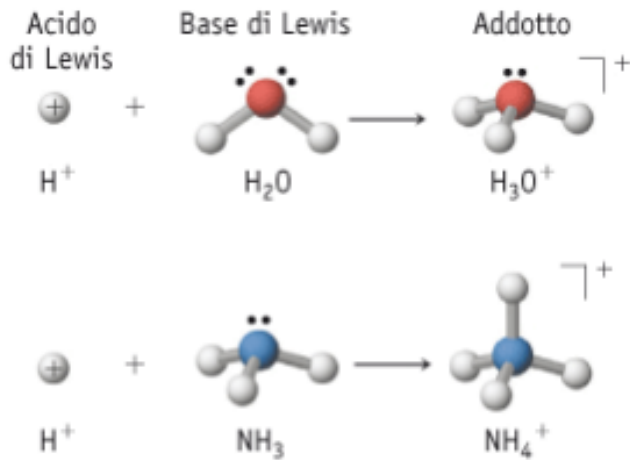
\includegraphics[width=8cm]{immagini/acidi_e_basi_di_lewis.png}
\end{figure}
